\documentclass[11pt,]{article}
\usepackage{array}
\usepackage{booktabs}
\usepackage{amsmath}
\usepackage{graphicx}
\usepackage{multirow, makecell, caption}
\usepackage[left=1.25in,top=1in,right=1in,bottom=1in]{geometry}
\newcommand*{\authorfont}{\fontfamily{phv}\selectfont}
\usepackage[]{mathpazo}


  \usepackage[T1]{fontenc}
  \usepackage[utf8]{inputenc}



\usepackage{abstract}
\renewcommand{\abstractname}{}    % clear the title
\renewcommand{\absnamepos}{empty} % originally center

\renewenvironment{abstract}
 {{%
    \setlength{\leftmargin}{0mm}
    \setlength{\rightmargin}{\leftmargin}%
  }%
  \relax}
 {\endlist}

\makeatletter
\def\@maketitle{%
  \newpage
%  \null
%  \vskip 2em%
%  \begin{center}%
  \let \footnote \thanks
    {\fontsize{18}{20}\selectfont\raggedright  \setlength{\parindent}{0pt} \@title \par}%
}
%\fi
\makeatother




\setcounter{secnumdepth}{0}


\usepackage{graphicx,grffile}
\makeatletter
\def\maxwidth{\ifdim\Gin@nat@width>\linewidth\linewidth\else\Gin@nat@width\fi}
\def\maxheight{\ifdim\Gin@nat@height>\textheight\textheight\else\Gin@nat@height\fi}
\makeatother
% Scale images if necessary, so that they will not overflow the page
% margins by default, and it is still possible to overwrite the defaults
% using explicit options in \includegraphics[width, height, ...]{}
\setkeys{Gin}{width=\maxwidth,height=\maxheight,keepaspectratio}

\title{Racially Concentrated Areas of Affluence:A Preliminary Investigation \thanks{Replication files are available on the author's Github account
(\url{http://github.com/tdamiano}). \textbf{Current version}: April 30,
2019; \textbf{Corresponding author}:
\href{mailto:egoetz@umn.edu}{\nolinkurl{egoetz@umn.edu}}}  }



\author{\Large Edward G. Goetz\vspace{0.05in} \newline\normalsize\emph{University of Minnesota}   \and \Large Anthony Damiano\vspace{0.05in} \newline\normalsize\emph{University of Minnesota}   \and \Large Rashad Williams\vspace{0.05in} \newline\normalsize\emph{University of Minnesota}  }


\date{}

\usepackage{titlesec}

\titleformat*{\section}{\normalsize\bfseries}
\titleformat*{\subsection}{\normalsize\itshape}
\titleformat*{\subsubsection}{\normalsize\itshape}
\titleformat*{\paragraph}{\normalsize\itshape}
\titleformat*{\subparagraph}{\normalsize\itshape}



\usepackage[style=apa]{biblatex}

\addbibresource{bib.bib}


\newtheorem{hypothesis}{Hypothesis}
\usepackage{setspace}

\makeatletter
\@ifpackageloaded{hyperref}{}{%
\ifxetex
  \PassOptionsToPackage{hyphens}{url}\usepackage[setpagesize=false, % page size defined by xetex
              unicode=false, % unicode breaks when used with xetex
              xetex]{hyperref}
\else
  \PassOptionsToPackage{hyphens}{url}\usepackage[unicode=true]{hyperref}
\fi
}

\@ifpackageloaded{color}{
    \PassOptionsToPackage{usenames,dvipsnames}{color}
}{%
    \usepackage[usenames,dvipsnames]{color}
}
\makeatother
\hypersetup{breaklinks=true,
            bookmarks=true,
            pdfauthor={Edward G. Goetz (University of Minnesota) and Anthony Damiano (University of Minnesota) and Rashad Williams (University of Minnesota)},
             pdfkeywords = {},
            pdftitle={Racially Concentrated Areas of Affluence:A Preliminary Investigation},
            colorlinks=true,
            citecolor=blue,
            urlcolor=blue,
            linkcolor=magenta,
            pdfborder={0 0 0}}
\urlstyle{same}  % don't use monospace font for urls

% set default figure placement to htbp
\makeatletter
\def\fps@figure{htbp}
\makeatother



% add tightlist ----------
\providecommand{\tightlist}{%
\setlength{\itemsep}{0pt}\setlength{\parskip}{0pt}}

\begin{document}

% \pagenumbering{arabic}% resets `page` counter to 1
%
% \maketitle

{% \usefont{T1}{pnc}{m}{n}
\setlength{\parindent}{0pt}
\thispagestyle{plain}
{\fontsize{18}{20}\selectfont\raggedright
\maketitle  % title \par

}

{
   \vskip 13.5pt\relax \normalsize\fontsize{11}{12}
\textbf{\authorfont Edward G. Goetz} \hskip 15pt \emph{\small University of Minnesota}   \par \textbf{\authorfont Anthony Damiano} \hskip 15pt \emph{\small University of Minnesota}   \par \textbf{\authorfont Rashad Williams} \hskip 15pt \emph{\small University of Minnesota}   

}

}








\begin{abstract}

    \hbox{\vrule height .2pt width 39.14pc}

    \vskip 8.5pt % \small

\noindent Racially/Ethnically Concentrated Areas of Poverty (RECAPs) have become
an official focus of policy attention for the U.S. Department of Housing
and Urban Development (HUD) through the 2015 rule regarding local
governments obligations to Affirmatively Further Fair Housing. In this
article, we argue for equal attention to the other end of the
segregation continuum, affluent White neighborhoods, or what we call
Racially Concentrated Areas of Affluence (RCAAs). We examine the
prevalence and characteristics of RCAAs in the 50 largest metropolitan
areas of the United States. Our findings show that RCAAs, as we define
them, are not as prevalent as RECAPs, accounting for an average of 2.2
percent of all tracts in the 50 largest metro areas compared with
RECAPs, which are an average of 4.7 percent of metro tracts. RCAAs are
more common in several metropolitan areas than RECAPs. The two phenomena
seem to be related; controlling for group size, the correlation between
metro area shares of RCAAs and RECAPs is moderately positive. We
conclude by offering reasons for focusing policy attention on RCAAs that
include acknowledging the various public policies that have created
these enclaves of advantage and the ways in which current and past
public policies have subsidized them.


    \hbox{\vrule height .2pt width 39.14pc}


\end{abstract}


\vskip 6.5pt


\noindent \doublespacing \hypertarget{introduction}{%
\section{Introduction}\label{introduction}}

Concentrations of poverty combined with racial segregation produce
conditions that have been the target of urban and housing policy since
the 1980s. Deconcentrating poverty was the objective behind HOPE VI,
Moving to Opportunity (MTO), and various HUD initiatives that focused on
dispersing subsidized households more widely throughout metropolitan
areas. The confluence of race and poverty is the specific target of
HUD's recent regulatory initiative related to Affirmatively Furthering
Fair Housing (AFFH). The 2015 AFFH rule requires local governments to
study what HUD calls ``Racially/Ethnically Concentrated Areas of
Poverty'' (RECAPs) to inform local efforts to further fair housing
goals. The orientation of much recent housing policy during this time
period has been to deconcentrate the poor and desegregate people of
color, either by facilitating or forcing their movement out of the
neighborhoods in which they predominate, or by redevelopment schemes
aimed at introducing more upscale housing and higher income residents
\autocite{goetzCtW2003}. Countless studies by academics of the dynamics
of high-poverty, segregated neighborhoods and the prospects for their
improvement have accompanied this strategy
\autocite{jargowsky1997poverty,sharkey2013}. The media, for their part,
have produced a steady stream of sensationalized reporting on the
``pathologies'' of these neighborhoods, especially during the 1980s and
1990s, fueling both academic attention and a policy focus
\autocite{sharkey2013}.

Curiously, although low-wealth communities of color have been thoroughly
problematized and portrayed as the most recognizable example of racial
and income segregation in the United States, relatively little attention
has been given to the other side of the segregation dynamic---the
affluent, White community. Racially Concentrated Areas of Affluence
(RCAAs) are not currently referenced in Federal housing policy, nor have
they been scrutinized to the extent that RECAPs have. However, patterns
of segregation in the United States show that of all racial groups,
Whites are the most severely segregated \autocite{feagin2014}. Research
also tells us that the segregation of affluence is greater than the
segregation of poverty \autocite{feagin2014}. The fact that segregation
of the poor and the wealthy is proceeding apace, confirms Sheryll
Cashin's \autocite*[p.~185]{cashin2004failures} observation that ``the
favored quarter, like the Black ghetto, represents an extreme of
American separatism.''

Concern about racially concentrated areas of affluence as an expression
of problematic separatism is largely absent from our national housing
policy agenda and the public imagination more broadly. The continued
elision of White neighborhoods of concentrated affluence and social
power within normative inquiry reinforces the decades-old tendency to
problematize low-income communities of color, while at the same time
sparing White neighborhoods and the advantages they embody from
examination of any kind. Analyses of segregation that disregard RCAAs
understate the degree to which advantage and disadvantage, opportunity
and inopportunity, and mobility and immobility are integrally linked.
Although our chief objective is not to exhaust the interconnections of
these divergent social formations, we see these linked dualities as the
normative compass guiding our inquiry into RCAAs. We also see our
project as contributing to the growing body of scholarship within the
relatively new field of critical whiteness studies. We contribute to
this work by empirically exploring not only the ``public and
psychological wage'' that whiteness confers
\autocite{du2017black,roediger1999wages} but also the material. In other
words, our concern is how whiteness---particularly in the neighborhood
context---confers unearned distributive advantages
\autocite{lipsitz2006possessive}.

In this article, we examine both racially concentrated poverty and
racially concentrated affluence in the largest 50 metropolitan areas in
the United States. Our purpose is to shed light on both extremes of
residential segregation in American urban areas. Our interest is
uncovering the extent of this settlement pattern by mapping the
geographic location of these neighborhoods, preliminarily testing
hypotheses about the prevalence and nature of RCAAs and assessing the
degree to which they correlate with other dimensions of metropolitan
growth dynamics (that is, overall segregation indices and economic and
demographic characteristics).

In this research, we conceptualize neighborhoods as occupying points in
a two-by-two field defined by race and affluence. In exhibit 1, the
vertical axis is defined by the racial makeup of neighborhoods, from
completely non-White to completely White. The horizontal axis is defined
by wealth from least to most affluent. RECAPs occupy the lower left
extreme of the plot, whereas RCAAs are the neighborhoods in the upper
right. Because of the high correlation between race and income in the
United States, we expect that metropolitan areas will present a
distribution of neighborhoods that resembles to some degree the
relationship depicted in exhibit 1; namely, that as neighborhood income
increases, the percentage of residents who are White also increases.

\begin{figure}
\includegraphics[width=4in]{./RCAP-RCAA-Continuum} \caption{Racially Concentrated Areas of Poverty and Affluence Continuum}\label{fig:fig1}
\end{figure}

\hypertarget{racially-concentrated-affluence-and-poverty}{%
\section{Racially Concentrated Affluence and
Poverty}\label{racially-concentrated-affluence-and-poverty}}

Residential segregation has long been a defining characteristic of
American metropolitan areas and a subject of extensive social science
and public policy concern. Although most indicators of racial
segregation show modest declines in recent years, segregation remains a
central characteristic of many metropolitan areas
\autocite{lichter2015toward,logan2011persistence}. Concentrations of
poverty, having abated somewhat during the 1990s, grew again with the
turn of the century \autocite{anacker2015kn}.

The ``costs'' of segregation have been carefully enumerated by many (for
example, Anderson, \autocite*{anderson2010}). For most scholars, the
focus has been on widespread and persistent patterns of racial
segregation in American communities and how these patterns create and
reinforce a range of inequalities. A large body of research has also
documented the negative impacts of concentrated poverty on economic and
social opportunities and outcomes. Racially concentrated areas of
poverty entrench these negative impacts for minority populations and
reinforce socio-economic disparities along racial lines. Inequalities in
affluence and income are among the most obvious costs of segregation:
gaps in wealth and income due to gaps in education and job-readiness
from discrimination and differences in educational experiences and
benefits of place. Inequalities in housing equity, housing conditions,
and lending and availability of credit are related outcomes of
residential segregation \autocite{lipsitz2006possessive}.

Economic inequalities are not the only costs of high levels of
segregation. Exposure to harmful environmental conditions and crime in
segregated, low-wealth communities combine with diminished public
services to make life more dangerous \autocite{hs2009hs}, leading to
inequalities in life expectancy between Whites and Blacks and rich and
poor \autocite{jackson2000relation,anderson2010}. Even the access to
critical types of social capital is unevenly distributed across
communities, leaving residents of low-wealth communities with social
networks that are less helpful in achieving upward mobility
\autocite*{briggs1998}. Strong patterns of segregation are worrisome
because they are ``structures of oppression'' \autocite{young2002}.
Segregation is a ``self-reinforcing dynamic''
\autocite{galster1999evolving} that exaggerates race and class
differences and reinforces discrimination.

Public policy, furthermore, is implicated in the creation and
maintenance of spatial inequality in American urban areas, whether it is
the role of Federal and local housing programs in producing segregated
communities of color, or the impact of local zoning, land use controls,
and systems of local public finance in creating and protecting areas of
White affluence. Despite this dual complicity, for policymakers (and
most social scientists) concerned with addressing problems of
segregation, the focus is typically on the conditions and dynamics
within segregated communities of color and low-wealth neighborhoods.
This focus has produced an overwhelming orientation of public policy
toward altering the pattern of residential settlement among people of
color and the poor. Our policies have, in fact, placed ``no onus on
Whites to adjust and contribute to a new multicultural ethos''
\autocite[p.~81]{cashin2004failures}.

Research shows, however, that economic segregation is increasing at both
extremes of the wealth distribution \autocite{reardon2014} and that the
segregation of Whites in the United States exceeds that of any other
racial group \autocite{feagin2014}. Indeed, some of the worried-about
``costs'' of residential segregation apply to the actions of affluent
Whites attempting to isolate from others. As Tilly
\autocite*{tilly1998durable} noted, the isolation of low-income
communities and people of color occurs against the backdrop of
opportunity hoarding, the corralling of resources for the exclusive
benefit of already advantaged groups. Just as segregation reinforces the
social locations of those already disadvantaged, it too reinforces the
tendency of the White and wealthy to legitimate and enclose their
advantages for in-group consumption \autocite{anderson2010}. For
example, Reardon and Bischoff \autocite*{reardon2014} suggested the
erosion of ``social empathy'' that results from close physical proximity
between the middle classes and the poor could enhance the likelihood of
``self-interested investments'' that serve narrow interests at the
expense of more universal social and economic needs. The converse may
also be true; support for more universal public goods declines under
conditions of segregation. As Anderson \autocite*[p.~61]{anderson2010}
noted: ``Whites favor tax limitations more strongly in more ethnically
diverse jurisdictions so they do not have to share their tax
contributions with other groups'' (see also the findings in Alesina et
al., \autocite*{alesina1999}).

Although Tilly, Anderson, and others refer to this dynamic as
opportunity hoarding, we argue that it is better understood as
``advantage hoarding.'' People who benefit from unjust socio-economic
relations and neighborhood exclusivity do not have to actively ``seize
the opportunity'' because neighborhood conditions confer automatic
benefits. Advantages such as high and rising property values, quality
schools, safety, and so on accrue merely through residence in such
neighborhoods.

Hoarding is but one of the many mechanisms that link the divergent
trajectories of marginalized neighborhoods on the one hand and exclusive
neighborhoods on the other. Some have argued that segregation leads to
high levels of land consumption in metropolitan areas, as the White and
the wealthy move ever outward to separate themselves from other segments
of society \autocite{cashin2004failures}. The willingness of Whites and
affluent families to pay for exclusivity increases land and housing
costs. Others point to the creation and maintenance of social divisions
resulting from segregation; the extreme separation of races leads to
greater fear of ``the other'' by both Blacks and Whites
\autocite{feagin2014}. Iris Marion Young \autocite*{young2002} argued
that social and political indifference is facilitated ``when privileged
classes live in separate political jurisdictions'' and are thus able to
keep resources and insulate themselves from the less fortunate.

Others point to how race and class segregation work in ways that obscure
the privileges of the favored. Again, as Young
\autocite*[p.208]{young2002} argued, ``segregation makes privilege
doubly invisible to the privileged'' by keeping disadvantage out of
sight and normalizing advantage. Anderson \autocite*{anderson2010} noted
that racial separation allows the favored group to enjoy advantages
without personally discriminating against the disadvantaged. According
to the argument, the pursuit of the favored group's well-being and the
enjoyment of the highest quality public and private services are
achieved in isolation. All this combines to insulate the favored group
and reduce their incentives to support services they do not see or use.
This contrasts with suburban Black middle-class neighborhoods, which
tend to be more economically diverse \autocite{pattillo2005black},
spending more of their tax revenues on redistributive policies at the
expense of commercially attractive public investments
\autocite{phelan1996race,anderson2010}. These realities are likely
becoming increasingly acute given growing economic inequality in the
United States during the past 30 years, which is largely a result of
increased income and wealth accumulation of the top end of the income
distribution \autocite{saez2013,shapiro2017}.

In recent years, a body of research has grown on the topic of the
so-called ``super-rich'' and what researchers are calling ``alpha
territories.'' Alpha territories are areas of global cities in which the
super-rich live and invest
\autocite{atkinson2017,burrows2014life,forrest2017}. This literature is
more an investigation of contemporary capitalism, the behavioral and
investment patterns of a global elite, and their impact on cities across
the world than it is an examination of residential segregation (for
example, Beaverstock, Hubbard, and Short, \autocite*{beaverstock2004};
Pow, \autocite*{pow2011living}; Rich \autocite*{rich2008}; and Hay and
Muller, \autocite*{hay2012tiny}).

Studies focusing on the segregation of affluence include the work of
Coulton et al \autocite*{coulton1996} on the relationship between
concentrated poverty and concentrated affluence. They found little
correlation at the metropolitan level, although they did note that MSAs
with higher levels of racial or ethnic segregation also saw high rates
of economic segregation. Massey and Eggers \autocite*{massey1993} also
looked at the segregation of affluence and poverty and their spatial
isolation from each other. They too found evidence that rates of racial
segregation influenced the level of poor-affluent segregation in the
1970s and 1980s. St.~John \autocite*{stjohn1999} examined the rate at
which affluent households (both Black and White) live in neighborhoods
where 50 percent or more of the households are affluent. St.~John's
analysis of 335 MSAs using 1990 census data shows that concentrations of
affluence were greater in metro areas with economic bases that had more
fully experienced restructuring away from durable goods manufacturing
and toward global finance and services. The study also shows that
greater income inequality and higher absolute levels of income in
metropolitan areas were associated with higher rates of concentrated
affluence. Like Coulton et al.~\autocite*{coulton1996} and Massey and
Eggers \autocite*{massey1993}, St.~John found that Black/White
segregation was related to the concentration of affluence. Lee and
Marlay \autocite*{lee2007right} provided a descriptive analysis of
affluent neighborhoods in the largest 100 U.S. metropolitan areas that
shows that the concept is robust to a range of different measures.

These previous studies of concentrated affluence are based on census
data from 2000 and earlier. Furthermore, although they suggest that
racial segregation and income segregation are related, they do not
examine the phenomenon of White affluence directly. Given the
meta-analysis by Jackson \autocite*{jackson2000relation} showing that
Whites more than Blacks benefit from concentrated affluence, we argue
the importance of investigating places of White affluence in the
American urban system. In the following analysis, we look at the two
extremes of racial and economic segregation in American metropolitan
areas: racially/ethnically concentrated areas of poverty (RECAPs) and
racially concentrated areas of affluence (RCAAs).

\hypertarget{methods}{%
\section{Methods}\label{methods}}

\hypertarget{data-and-variables}{%
\subsection{Data and Variables}\label{data-and-variables}}

All data used in our analyses originate from the American Community
Survey (ACS) 2012--2016 5-year estimate. We use several variables from
the ACS that depict the economic and demographic characteristics of
individuals and households and the characteristics of the housing stock.
All measures are at the census tract level. Our study covers the largest
50 metropolitan areas in the United States. We summarize our findings on
concentrated poverty and affluence by region. We do so for ease of
presentation, but also because regions capture important differences in
urban development history in the United States, and the evidence shows
that patterns of segregation vary significantly by region. Jargowsky
\autocite*{jargowsky1997poverty}, for example, showed that
concentrations of poverty have varied by region, with the phenomenon
growing first in the Midwest and Northeast and then spreading to other
areas. Massey and Denton \autocite*{massey1989hs} and Denton
\autocite*{denton1994african} demonstrated that rates of segregation and
hypersegregation of Blacks and Hispanics have also varied significantly
by region, with Northeast and Midwest metropolitan areas scoring highest
on most indices of residential segregation.

Defining Racially/Ethnically Concentrated Areas of Poverty (RECAPs). We
use a well-established set of criteria for identifying RECAPs to define
them in our work. According to HUD, a RECAP is a census tract in which
more than 40 percent of the residents have incomes less than the Federal
poverty level and more than 50 percent of the residents of the census
tract are people of color (HUD, 2011). We considered individuals to be
people of color if they did not identify themselves as ``Not Hispanic or
Latino: White Alone.'' We could find no theoretical or empirical
justification for the racial threshold in the RECAP definition, which
appears to be simply an arbitrary level adopted by the Federal
government. The justification for the poverty threshold, however, does
have an empirical basis. Jargowsky and Bane
\autocite*{jargowsky1991ghetto} argued that the 40-percent poverty
threshold is confirmed by their field research in metropolitan areas
across the country. Neighborhoods that knowledgeable local informants
regarded as ghettos, barrios, and slums consistently matched census
tracts that had poverty rates of 40 percent or more. Since then, the
40-percent threshold has been widely adopted and has been argued to be
the degree of neighborhood poverty above which disadvantage accelerates.

\hypertarget{defining-racially-concentrated-areas-of-affluence-rcaas}{%
\subsection{Defining Racially Concentrated Areas of Affluence
(RCAAs)}\label{defining-racially-concentrated-areas-of-affluence-rcaas}}

Our objective in defining RCAAs is to mirror as much as possible the
dimensions and methods that constitute the RECAP definition. To think of
these phenomena as two ends of the same continuum requires conceptual
and operational symmetry. We seek to incorporate four important
characteristics of the RECAP definition that into the RCAA definition.
First, and most obviously, the neighborhood is defined both by race and
by income. Second, to the extent possible, we wish to identify an
empirical justification for the race and income thresholds we use
(noting as we have previously that the RECAP definition itself fails
this standard for race). Third, we seek a definition that is invariant
across metropolitan areas. The RECAP definition uses the national
poverty level and does not adjust for cost of living across metro areas.
It also uses a uniform standard of 50 percent people of color that does
not adjust for the degree of racial diversity by metro area. Finally, we
seek to mirror the RECAP definition by avoiding a definition that
predetermines the prevalence of RCAAs across or within metro areas. This
aspect of the definition is reflected in the use of absolute measures of
income and race rather than defining these neighborhoods as occupying
some percentage of the total distribution of neighborhoods.

We posit that, in the same way neighborhood disadvantage is associated
with concentrated poverty and high concentrations of people of color,
conversely, distinct advantages are associated with residence in
affluent, White communities. We hypothesize that the returns of living
in predominantly White and affluent neighborhoods are nonlinear and
accelerate at the high end. What we seek in a definition of RCAAs is the
combination of the level of whiteness and affluence at the neighborhood
scale at which returns accelerate. We use census tract median home value
as a proxy for neighborhood advantage. Home values represent a
reasonable indicator of neighborhood advantage because they not only
capture the quality of the housing stock, they also capture neighborhood
characteristics associated with advantages, including good schools, low
crime, job proximity, and environmental quality. Finally, and most
obviously, they are themselves a form of wealth.

We conduct nonlinear regression analysis to investigate the impact of
percent White and median household income on home values and include a
variety of controls associated with neighborhood advantage, including
share of adults with a college degree, home ownership rate, and whether
the tract was in a central city. We also included a metro area fixed
effect to account for systematic differences between metro areas. We
operationalize share White as a categorical variable broken into 5
percentage-point increments and interact that variable with median
household income. The analysis, summarized in the appendix, describes a
non-linear relationship between percent White and home values, with an
inflection point estimated at 80 percent (see appendix for details of
this step).

Finding a threshold for concentrated affluence using these methods
proved more difficult as the model estimated a constant, linear return
to household incomes. Without a strong empirical justification for an
income threshold, we turn to previous studies of concentrated affluence.
Unfortunately, the literature provides no consistent guide for defining
the concept. Lee and Marlay \autocite*{lee2007right}, for example,
operationalized affluent neighborhoods as those in the highest 2 percent
in income across the 100 largest metro areas they study. Solari's
\autocite*{solari2012} study of concentrated affluence defines such
neighborhoods as the top 10 percent within a metro area's
neighborhood-income distribution. These definitions, however, violate
our fourth guideline for a definition of RCAAs and are inconsistent with
the methods used to define RECAPs.

Massey and Eggers used family income of more than \$30,000 in 1979 as
the basis of their examination of affluence in the 1970s. This was
slightly more than 50 percent above the national family median income in
1979. In his study of concentrated affluence, St.~John used a threshold
equal to four times the poverty rate. This produced an income level
around \$100,000, although St.~John used a cost of living index that
produced a threshold that varied by metro area (and therefore violates
our third guideline and is inconsistent with the methods used to define
RECAPs).

The greatest convergence in previous research on an income level to
define affluence puts the threshold at roughly two times the national
median. Coulton et al.~\autocite*{coulton1996}, for example, used a 1990
median family income of over \$75,000, which was just over two times the
national median in the 1990 census. They argued that such a standard was
consistent with other research on affluence, citing Kosters and Ross
\autocite*{kosters1988shrinking} and Blackburn and Bloom
\autocite*{blackburn1985h}.

We adopt a median household income of \$125,000 as our standard. This
level is, like Coulton et al., slightly greater than two times the
national median in 2016. To achieve our other objective in establishing
a definition of RCAA that is symmetrical with that of the RECAP, we use
a constant measure of income and do not adjust for cost of living. Thus,
our definition of RCAA is a census tract in which 80 percent or more of
the population is White and has a median income of at least \$125,000.

\hypertarget{analysis}{%
\section{Analysis}\label{analysis}}

The distribution of census tracts along the two dimensions that define
RECAPs and RCAAs is shown for a sample of metro areas in figure 2.
Rather than being linear, as depicted theoretically in figure 1, the
relationship between percent White and income in census tracts is in
fact curvilinear in most metropolitan areas. This is due to one
variable, percent White, having an upward limit of 100, whereas the
other variable, income, has no upper bound (although is top-coded at
\$250,000). The curvilinear form of this relationship is common to most
of the metropolitan areas in our sample and is shown in both the
Pittsburgh and Salt Lake City plots. In a small number of metro areas,
the relationship is not very distinct. As shown for San Jose, the
scatterplot is much more diffuse.

\begin{figure}
\centering
\includegraphics{GDW-RCAA-2019_files/figure-latex/fig2-1.pdf}
\caption{Income and Racial Distribution for sample MSAs(RECAPs/RCAAs
Highlighted)}
\end{figure}

\hypertarget{segregation-by-race}{%
\subsection{Segregation by Race}\label{segregation-by-race}}

Table 1 shows the isolation index for Whites and people of color in our
50 metropolitan areas sample. The isolation index measures the degree to
which a person of a particular category is surrounded by members of the
same group \autocite{massey1989hs}. In 70 percent of the metro areas in
our sample, Whites lived in more segregated neighborhoods compared to
people of color. Average White isolation in our sample was 25 percent
higher than the isolation for people of color. Overall, the typical
White person lived in a neighborhood that was 71 percent White, whereas
a typical person of color in our sample lived in a neighborhood that was
57 percent people of color. The 10 metro areas with the highest levels
of racial isolation of Whites were in the Midwest or Northeast and, not
surprisingly given the dynamics of the isolation index, also tended to
have larger White populations. Conversely, metro areas with the highest
racial isolation for people of color tended to be in the South and West
regions and tended to have larger shares of non-White populations.

\begin{table}[t]

\caption{\label{tab:table1}Average Metro Area Racial Isolation by Region}
\centering
\begin{tabular}{lccccc}
\toprule
\multicolumn{2}{c}{ } & \multicolumn{2}{c}{White} & \multicolumn{2}{c}{People of Color} \\
\cmidrule(l{3pt}r{3pt}){3-4} \cmidrule(l{3pt}r{3pt}){5-6}
Region & N & mean & sd & mean & sd\\
\midrule
Midwest & 10 & 0.82 & (0.04) & 0.53 & (0.1)\\
Northeast & 7 & 0.81 & (0.07) & 0.53 & (0.11)\\
South & 22 & 0.68 & (0.08) & 0.60 & (0.1)\\
West & 11 & 0.61 & (0.12) & 0.58 & (0.15)\\
\textbf{Total} & \textbf{50} & \textbf{0.71} & \textbf{(0.11)} & \textbf{0.57} & \textbf{(0.12)}\\
\bottomrule
\end{tabular}
\end{table}

Another way to document racial concentrations is to analyze the shares
of Whites and people of color that live in racially/ethnically
concentrated census tracts. Table 2 shows that in every region, larger
percentages of Whites live in majority White tracts compared to the
share of people of color who live in majority POC tracts. This pattern
holds in the aggregate, but also for 90 percent of the individual metro
areas in our sample, greater shares of Whites live in majority White
neighborhoods compared to people of color. More than 80 percent of
Whites in our sample metro areas live in census tracts that are majority
White compared with 60 percent of people of color.

\begin{table}[t]

\caption{\label{tab:table2}Average Metro Area Racial Concentration by Region }
\centering
\begin{tabular}{lccccccc}
\toprule
\multicolumn{2}{c}{ } & \multicolumn{2}{c}{\makecell[c]{Share POC living in\\majority POC tracts}} & \multicolumn{2}{c}{\makecell[c]{Share of Whites living in\\majority White tracts}} & \multicolumn{2}{c}{\makecell[c]{Share of Whites in 80+\\White tracts}} \\
\cmidrule(l{3pt}r{3pt}){3-4} \cmidrule(l{3pt}r{3pt}){5-6} \cmidrule(l{3pt}r{3pt}){7-8}
Region & N & mean & sd & mean & sd & mean & sd\\
\midrule
Midwest & 10 & 51.0 & (12.7) & 93.6 & (3.2) & 67.8 & (10.8)\\
Northeast & 7 & 50.7 & (14.5) & 91.2 & (6.7) & 65.3 & (17.7)\\
South & 22 & 61.0 & (14.2) & 79.0 & (12.9) & 33.0 & (16.6)\\
West & 11 & 60.6 & (26.4) & 71.2 & (19.5) & 22.9 & (20.2)\\
\textbf{Total} & \textbf{50} & \textbf{57.5} & \textbf{(17.5)} & \textbf{81.9} & \textbf{(15)} & \textbf{42.3} & \textbf{(24.3)}\\
\bottomrule
\end{tabular}
\end{table}

Table 2 also presents White racial concentration using our more
conservative 80-percent threshold. In the average metropolitan area in
the Northeast, for example, two-thirds of all Whites live in census
tracts in which 80 percent or more of the residents are also White. In
contrast, in Western metro areas the average is less than one-fourth of
Whites. In 19 of the sample metro areas the share of Whites living in
tracts with 80 percent or more Whites is greater than the share of
people of color living in tracts with 50 percent or more people of
color.

\hypertarget{income-concentration}{%
\subsection{Income Concentration}\label{income-concentration}}

Our analysis shows that 36 percent of metro areas had higher rates of
concentrated affluence compared with concentrated poverty. We find 16
percent more areas of concentrated affluence compared to areas of
concentrated poverty (2,297 tracts and 1,983 tracts respectively).
However, the distribution of concentrated affluence is skewed toward
fewer metro areas leading to higher average amounts of concentrated
poverty compared to concentrated affluence in our sample.

\begin{table}[t]

\caption{\label{tab:table3}Average Metro Area Income Concentration by Region}
\centering
\begin{tabular}{lccccc}
\toprule
\multicolumn{2}{c}{ } & \multicolumn{2}{c}{\makecell[c]{Share Tracts w/\\Con. Affluence}} & \multicolumn{2}{c}{\makecell[c]{Share Tracts w/\\Con. Poverty}} \\
\cmidrule(l{3pt}r{3pt}){3-4} \cmidrule(l{3pt}r{3pt}){5-6}
Region & N & mean & sd & mean & sd\\
\midrule
Midwest & 10 & 2.71 & (1.41) & 9.20 & (4.14)\\
Northeast & 7 & 4.95 & (4.46) & 5.13 & (2.33)\\
South & 22 & 4.27 & (5) & 5.33 & (4.23)\\
West & 11 & 7.00 & (8.11) & 2.27 & (1.6)\\
\textbf{Total} & \textbf{50} & \textbf{4.66} & \textbf{(5.39)} & \textbf{5.40} & \textbf{(4.14)}\\
\bottomrule
\end{tabular}
\end{table}

Metro areas with the highest rates of concentrated poverty like Memphis,
TN, Milwaukee, WI, and Detroit, MI, tended to be in the South and
Midwest; metro areas in the Midwest, on average, had the lowest rates of
concentrated affluence and the highest rates of concentrated poverty. In
contrast, on average, metro areas in the West showed the highest rates
of concentrated affluence and the lower rates of concentrated poverty.
One metro area, Salt Lake City, UT, had zero areas of concentrated
poverty.

\hypertarget{racially-concentrated-areas-of-affluence-and-poverty}{%
\section{Racially Concentrated Areas of Affluence and
Poverty}\label{racially-concentrated-areas-of-affluence-and-poverty}}

In the previous section, we analyzed the prevalence and degree of racial
or ethnic concentrations and income concentrations separately. In this
section, we will directly explore both ends of the income/racial
distribution and compare the prevalence and characteristics of RCAAs and
RECAPs.

Table 4 shows the distribution of RCAAs and RECAPs summarized by region.
We find that in our sample, RCAAs are more common in the Midwest and
Northeast. RECAPs are most common in the Midwest. The West region has,
on average, the fewest RCAAs and the fewest RECAPs despite being the
most racially diverse region in our sample.

\begin{table}[t]

\caption{\label{tab:table4}Average Share of Census Tracts that Qualify as RCAA and RECAP by Region}
\centering
\begin{tabular}{lccccc}
\toprule
\multicolumn{2}{c}{ } & \multicolumn{2}{c}{RCAA} & \multicolumn{2}{c}{RECAP} \\
\cmidrule(l{3pt}r{3pt}){3-4} \cmidrule(l{3pt}r{3pt}){5-6}
Region & N & mean & sd & mean & sd\\
\midrule
Midwest & 10 & 2.2 & (1) & 7.4 & (4.1)\\
Northeast & 7 & 3.6 & (2.8) & 4.2 & (2.2)\\
South & 22 & 2.1 & (1.4) & 4.9 & (4.3)\\
West & 11 & 1.6 & (1.5) & 2.0 & (1.7)\\
\textbf{Total} & \textbf{50} & \textbf{2.2} & \textbf{(1.7)} & \textbf{4.7} & \textbf{(3.9)}\\
\bottomrule
\end{tabular}
\end{table}

Tables 5 and 6 shows the metro areas with the highest rates of RCAAs and
RECAPs. Metro areas with high rates of RCAAs tend to be in Whiter metro
areas. The list of metro areas with the highest rates of RECAPs is
dominated by rustbelt metro areas like Milwaukee, Detroit, Cleveland,
and Buffalo. Chicago is the only city that appears on both lists. Salt
Lake City was the only metro area that had no RECAP, and Las Vegas was
the only metro area in our sample without any RCAA.

\begin{table}[t]

\caption{\label{tab:table5}Metro Areas w/ Higheset RCAA Concentrations}
\centering
\begin{tabular}{clcc}
\toprule
Rank & Metro Name & N RCAA & Share of MSA Tracts\\
\midrule
1 & Boston-Cambridge-Newton, MA-NH & 79 & 8.8\\
2 & Denver-Aurora-Lakewood, CO & 33 & 5.4\\
3 & New York-Newark-Jersey City, NY-NJ-PA & 229 & 5.0\\
4 & Washington-Arlington-Alexandria, DC-VA-MD-WV & 65 & 4.9\\
5 & Philadelphia-Camden-Wilmington, PA-NJ-DE-MD & 68 & 4.7\\
\addlinespace
6 & Baltimore-Columbia-Towson, MD & 28 & 4.2\\
7 & Raleigh, NC & 9 & 4.0\\
8 & Nashville-Davidson--Murfreesboro--Franklin, TN & 15 & 4.0\\
9 & Minneapolis-St. Paul-Bloomington, MN-WI & 30 & 3.8\\
10 & Chicago-Naperville-Elgin, IL-IN-WI & 74 & 3.4\\
\bottomrule
\end{tabular}
\end{table}

\begin{table}[t]

\caption{\label{tab:table6}Metro Areas w/ Highest RECAP Concentrations}
\centering
\begin{tabular}{clcc}
\toprule
Rank & Metro Name & N RECAP & Share of MSA Tracts\\
\midrule
1 & Memphis, TN-MS-AR & 52 & 21.7\\
2 & Milwaukee-Waukesha-West Allis, WI & 58 & 13.6\\
3 & Detroit-Warren-Dearborn, MI & 168 & 13.1\\
4 & Cleveland-Elyria, OH & 81 & 12.8\\
5 & New Orleans-Metairie, LA & 39 & 9.9\\
\addlinespace
6 & Phoenix-Mesa-Scottsdale, AZ & 80 & 8.2\\
7 & Buffalo-Cheektowaga-Niagara Falls, NY & 23 & 7.9\\
8 & Birmingham-Hoover, AL & 17 & 6.5\\
9 & Chicago-Naperville-Elgin, IL-IN-WI & 135 & 6.1\\
10 & Oklahoma City, OK & 21 & 5.8\\
\bottomrule
\end{tabular}
\end{table}

Table 7 shows the average concentration of White affluent households
living in RCAAs and the average concentration of poor POC living in
RECAPs. In our 10 Midwestern metro areas, for example, just 7.5 percent
of affluent Whites lived in RCAAs. In those same metro areas, 24.8
percent of people of color under the poverty line lived in RECAPs. These
regional figures mirror the patterns in exhibit 6. On average, metro
areas in the Northeast and the Midwest had the highest shares of
affluent Whites living in RCAAs and poor people of color living in
RECAPs. The West, while being quite affluent overall, showed the lowest
rates of affluent Whites living in areas of concentrated White
affluence. Across all metro areas, the rate at which people of color
below the poverty line live in RECAPs (15.6) is more than twice the rate
at which White affluent households live in RCAAs (6.8).

\begin{table}[t]

\caption{\label{tab:table7}Concentration of White Affluence and Poor POC in RCAAs and RECAPs}
\centering
\begin{tabular}{lccccc}
\toprule
\multicolumn{2}{c}{ } & \multicolumn{2}{c}{Share Poor POC in RECAP} & \multicolumn{2}{c}{Share White Aff. HH in RCAA} \\
\cmidrule(l{3pt}r{3pt}){3-4} \cmidrule(l{3pt}r{3pt}){5-6}
Region & N & mean & sd & mean & sd\\
\midrule
Midwest & 10 & 24.8 & (11.2) & 7.5 & (2.7)\\
Northeast & 7 & 19.6 & (9.9) & 9.9 & (5.3)\\
South & 22 & 14.6 & (7.3) & 6.7 & (3.7)\\
West & 11 & 6.9 & (5) & 4.3 & (3.7)\\
\textbf{Total} & \textbf{50} & \textbf{15.6} & \textbf{(10)} & \textbf{6.8} & \textbf{(4)}\\
\bottomrule
\end{tabular}
\end{table}

\hypertarget{characteristics-of-recaps-and-rcaas}{%
\subsection{Characteristics of RECAPs and
RCAAs}\label{characteristics-of-recaps-and-rcaas}}

Comparing the income characteristics of RECAPs and RCAAs with the
average tract in their respective metro areas, we find that, on average,
RCAA tracts have more than twice the median household income of the
average tract in their metro area.

As expected, poverty rates in RCAAs are also significantly lower and
are, on average about 20 percent of a typical tract. On average, RCAAs
tracts are more income homogenous than RECAPs. The average RCAA in our
sample was 57 percent affluent, whereas the average RECAP had a poverty
rate of 48 percent. At the same time, RECAPs tended to be larger
outliers in terms of poverty rate from their respective metro areas than
RCAAs were in terms of affluence. The typical RCAA tract had a rate of
affluence 3.2 times that of a typical tract, whereas RECAPs on average
had a poverty rate 3.2 times that of a typical tract. The figures
presented in table 8 did not vary significantly by region.

\begin{table}[t]

\caption{\label{tab:table8}Average Income Characteristics of RCAAs and RECAPs}
\centering
\begin{tabular}{lccc}
\toprule
  & All Tract Average & RCAA Average & RCAP Average\\
\midrule
Median HH Income & \$64,589 & \$147,719 & \$23,071\\
Pct. Affluent & 17.8 & 57.2 & 2.9\\
Pct. Poverty & 15 & 3.2 & 47.9\\
\bottomrule
\end{tabular}
\end{table}

Table 9 details the racial breakdown of RCAAs and RECAPs and how the
racial characteristics compare with typical metro area tracts. By
definition, little racial variation occurs within RCAAs; RCAAs look the
same across all regions. RECAPs, however, show a much wider range of
racial characteristics. In the Midwest and the South, RECAPs are
majority Black (65 percent and 59 percent Black, respectively). In the
West, Hispanics are the largest racial/ethnic group in RECAPs, and
northeastern RECAPs are a mixture.

\begin{table}[t]

\caption{\label{tab:table9}Average Racial Characteristics of RCAAs and RECAPs}
\centering
\begin{tabular}{lccc}
\toprule
  & All Tract Average & RCAA Average & RCAP Average\\
\midrule
Pct. Asian & 5.6 & 4.2 & 4.3\\
Pct. Black & 16.5 & 1.9 & 49.9\\
Pct. Hispanic & 16.1 & 4.2 & 26.1\\
Pct. White & 58.6 & 87.5 & 16.4\\
\bottomrule
\end{tabular}
\end{table}

\hypertarget{geography-of-rcaas-and-recaps}{%
\subsection{Geography of RCAAs and
RECAPs}\label{geography-of-rcaas-and-recaps}}

On average, RCAA tracts are farther from the urban core than the average
census tract in a region and much farther away from the core compared to
the typical RECAP (see table 10). A typical RCAA in our sample is more
than twice as far away from the core as the typical RECAP. RECAPs in our
sample were also twice as dense on average as the typical metro area
tract and more than four times as dense as the typical RCAA. RCAAs are
more likely to be in suburban areas compared to the typical tracts,
whereas RECAPs are almost 2.5 times more likely to be in central cities.

\begin{table}[t]

\caption{\label{tab:table10}Distance from Central Business District and Population Density}
\centering
\begin{tabular}{lccc}
\toprule
  & All Tract Average & RCAA Average & RCAP Average\\
\midrule
Dist. from Core & 15.5 & 16.6 & 7.8\\
Pop Density & 5,131.6 & 2,283.2 & 9,703.7\\
Share located in Central CIty & 30.8 & 19.2 & 74.6\\
\bottomrule
\end{tabular}
\end{table}

Some metro areas deviated from this central city/suburban dynamic
between RCAAs and RECAPs. Most RECAPs were in suburban areas in the
Riverside, CA; Miami, FL; Louisville, KY; and Virginia Beach, VA metro
areas. Conversely, some metro areas had most of their RCAAs in the
central city including the Los Angeles, CA; Charlotte, NC; New Orleans,
LA; Tampa, FL; and Virginia Beach, VA.

Figure 3 maps four representative metro areas and highlights the
location of RCAAs and RECAPs. We see a common pattern of RECAPs
clustered in central cities, which is consistent with other research
\autocite{jargowsky1997poverty}. The ``classic'' pattern of central city
RECAPs and suburban RCAAs is shown in the map of Minneapolis and
St.~Paul, MN. Los Angeles, in contrast, shows a mix of RCAAs and RECAPs
within the central city boundaries. In some metro areas like St.~Louis,
MO and Chicago, IL, we also observe a directional dividing line between
RCAAs and RECAPs consistent with patterns of racial segregation in these
metro areas.

\begin{figure}
\centering
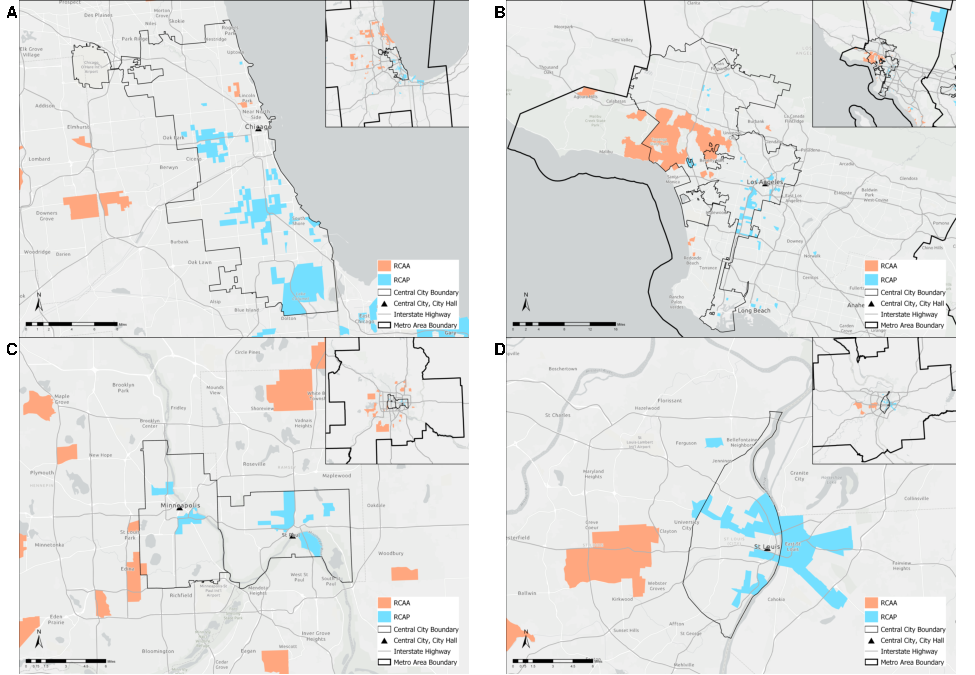
\includegraphics{GDW-RCAA-2019_files/figure-latex/fig3-1.pdf}
\caption{Mapping RCAAs and RECAPs - From left to right, (A) Chicago, (B)
Los Angeles, (C) Minneapolis-St.~Paul, (D) St.~Louis}
\end{figure}

\hypertarget{correlation-between-rcaas-and-recaps}{%
\subsection{Correlation between RCAAs and
RECAPs}\label{correlation-between-rcaas-and-recaps}}

In the previous section, we analyzed and compared different
characteristics of RCAAs and RECAPs compared with the typical
neighborhood. In this section, we examine whether the prevalence of
RECAPs and RCAAs is correlated. For this preliminary analysis, we began
with a scattergram that features the share of metro area tracts that
qualify as RCAAs on the x-axis and the share of tracts that qualify as
RECAPs on the y-axis (exhibit 13). The lines on the scattergram
represent the median values of share RCAA (1.7\%) and share RECAP
(3.9\%) of our sample respectively. One can see much greater variation
in the prevalence of RECAPs across metro areas (measured as a percentage
of all tracts within a region). The range would seem greater except that
the biggest outlier, Memphis, TN, is not pictured in the diagram because
it is so out of scale with the rest of the metro areas in our sample.
Following Memphis, the Midwestern cities of Milwaukee, WI, Cleveland,
OH, and Detroit, MI have the highest percentage of tracts meeting the
RECAP definition. Western cities typically rank low in prevalence of
RECAPs. The range in the prevalence of RCAAs is much more limited, with
Boston, MA standing out with the highest percentage. Cities appearing in
the upper right quadrant rank relatively high on both RECAPs and RCAAs.

\begin{figure}
\centering
\includegraphics{GDW-RCAA-2019_files/figure-latex/fig4-1.pdf}
\caption{Relationship between RCAAs and RECAPs}
\end{figure}

In table 11, we create a simple typology that places the 50 metro areas
in our sample into one of four categories based on whether their share
of each neighborhood type is above or below the median value for our
sample. This results in four mutually exclusive categories. First,
Low/Low metro areas have below the median percentage of RCAAs and
RECAPs. High/High metro areas have shares that qualified as RCAAs as
well as RECAPs above the median. The off-diagonal categories are metro
areas that have high levels of one type of and low levels of the other.

\begin{table}[t]

\caption{\label{tab:table11}Correlation in Prevalence of RECAPs and RCAAs}
\centering
\fontsize{7}{9}\selectfont
\begin{tabular}{l|l|l}
\hline
Cat & Low.RCAA & High.RCAA\\
\hline
High-RECAP & \makecell[l]{Birmingham-Hoover, AL\\                 Buffalo, NY\\                 Cleveland, OH\\                 Indianapolis, IN\\                 Jacksonville, FL\\                 Las Vegas, NV\\                 Memphis, TN\\                 Milwaukee, WI\\                 New Orleans, LA\\                 Oklahoma City, OK\\                 Sacramento, CA\\                 St. Louis, MO\\                 San Antonio, TX} & \makecell[l]{Austin, TX\\                 Baltimore, MD\\                 Boston, MA\\                 Charlotte, NC\\                 Denver, CO\\                 Louisville, KY\\                 Minneapolis-St. Paul, MN\\                 Nashville, TN\\                 Portland, OR\\                 Raleigh, NC\\                 Richmond, VA\\                 San Diego, CA\\                 San Francisco-Oakland, CA\\                 Washington, DC}\\
\hline
Low-RECAP & \makecell[l]{Los Angeles, CA\\                 Miami, FL\\                 Orlando, FL\\                 Pittsburgh, PA\\                 Providence, MA\\                 Riverside-San Bernardino, CA\\                 Salt Lake City, UT\\                 San Jose, CA\\                 Seattle, WA\\                 Tampa, FL\\                 Virginia Beach, VA} & \makecell[l]{Atlanta, GA\\                 Chicago, IL\\                 Columbus, OH\\                 Dallas-Fort Worth, TX\\                 Detroit, MI\\                 Hartford, CT\\                 Houston, TX\\                 Kansas City, MO\\                 New York, NY\\                 Philadelphia, PA\\                 Phoenix, AZ}\\
\hline
\end{tabular}
\end{table}

We find strong regional trends in this categorization. Most of the metro
areas in the High/High category are rust belt metro areas in the Midwest
and Northeast. The category includes the largest cities in our sample.
New York, Chicago, Houston, Philadelphia, and Phoenix are five of the
six most populous central cities in the country and their metro areas
are above the median in both RCAAs and RECAPs. There are no Western
cities in the High/High category.

The Low/Low category contains an over-representation of metro areas from
the West and no Midwest metro areas at all. In contrast to the pattern
of large central cities have high rates of both RCAAs and RECAPs, Los
Angeles is in the Low/Low category. These are some of the most racially
diverse metro areas in our sample like the Los Angeles, CA MSA, which
was only 30 percent White in 2015.

\begin{table}[t]

\caption{\label{tab:table12}Distance from Central Business District and Population Density}
\centering
\begin{tabular}{l>{\centering\arraybackslash}p{2.5cm}>{\centering\arraybackslash}p{2.5cm}>{\centering\arraybackslash}p{2.5cm}>{\centering\arraybackslash}p{2.5cm}>{\centering\arraybackslash}p{2.5cm}}
\toprule
Region & High-RCAA High-RCAP & High-RCAA Low-RCAP & Low-RCAA High-RCAP & Low-RCAA Low-RCAP & Total\\
\midrule
Midwest & 40.0\%  (4) & 10.0\%  (1) & 50.0\%  (5) & 0.0\%  (0) & 100.0\% (10)\\
Northeast & 42.9\%  (3) & 14.3\%  (1) & 14.3\%  (1) & 28.6\%  (2) & 100.0\%  (7)\\
South & 18.2\%  (4) & 36.4\%  (8) & 27.3\%  (6) & 18.2\%  (4) & 100.0\% (22)\\
West & 0.0\%  (0) & 36.4\%  (4) & 18.2\%  (2) & 45.5\%  (5) & 100.0\% (11)\\
\textbf{Total} & \textbf{22.0\% (11)} & \textbf{28.0\% (14)} & \textbf{28.0\% (14)} & \textbf{22.0\% (11)} & \textbf{100.0\% (50)}\\
\bottomrule
\end{tabular}
\end{table}

Metro areas that had low levels of RCAAs and high levels of RECAPs,
unsurprisingly tended to be poorer metro areas with larger shares of
people of color including Memphis, TN, and New Orleans, LA. This
category also includes metro areas with struggling central cities such
as Buffalo, Cleveland, Milwaukee, and St.~Louis. Conversely, the
high-RCAA/low-RECAP category contains six of the 10 wealthiest
metropolitan areas such as San Francisco, Washington, D.C., Boston, and
Portland. This category also includes the only Midwestern metro area
that registered a low number of RECAPs, Minneapolis-St.~Paul. Exhibit 14
lists all metro areas in the four quadrants, and exhibit 15 summarizes
the findings by region

\hypertarget{accounting-for-group-size}{%
\subsection{Accounting for Group Size}\label{accounting-for-group-size}}

Measures of concentration like RCAA and RECAP are significantly
correlated with group size. That is, the prevalence of RCAAs and RECAPs
depend in part on the overall share of people within a metro area who
are White and affluent on the one hand, and of color and poor on the
other. We found simple bivariate correlations of 0.72 for RCAAs and 0.46
for RECAPs\footnote{Variables transformed using an inverse hyperbolic
  sine transformation to normalize data. We used this rather than a
  simple log transformation due to the fact that the inverse hyperbolic
  sine transformation is defined at zero.}. As a test of robustness and
to better understand the relationship between RCAAs and RECAPs, we
performed two OLS regressions to control for the group size of White
affluent households and poor people of color using inverse hyperbolic
sine transformed variables to increase normality and compared the
standardized residuals from each equation. This allowed us to begin to
understand how group size affects RCAAs and RECAPs and to chart a more
valid analysis of the correlation between these two phenomena.

The equations for each type of segregation are below:

\[ MetroShareRCAA = \beta_0 + \beta_1ShareMetroWhiteAffluent + \epsilon \]
\[ MetroShareRECAP = \beta_0 + \beta_1ShareMetroPOCPoor + \epsilon \]

Without controlling for group size, we find little, if any, correlation
between metro areas that have high rates of RCAAs and RECAPs (-0.07).
After controlling for group size, we find a stronger albeit still
moderate positive correlation between metro areas' shares of RCAAs and
RECAPs (0.35, p \textless{}0.05).

\hypertarget{conclusion}{%
\section{Conclusion}\label{conclusion}}

The investigation of RCAAs, we argue, is necessary to achieve a fuller
understanding of inequality and segregation in American metropolitan
areas. Although public policy in the United States focuses on and
problematizes RECAPs---the confluence of large minority populations and
poverty---such concentrations are mirrored by exclusionary enclaves of
White affluence. These enclaves represent a second form of extreme
segregation in American metropolitan areas.

What is the value added of investigating RCAAs? We suggest four reasons
for focusing on RCAAs. In addition to the extensive research that has
focused on the damage to one's life chances from living in an RECAP
(that is, the ``neighborhood effects'' literature), some scholars have
focused on the inherent problematic nature of residential segregation
and the importance of diversity for well-functioning communities (in
both a social and political sense; Anderson, \autocite*{anderson2010}).
In this argument, the reality of intense segregation damages the larger
polity by making intergroup relations problematic, and by creating and
intensifying cross-group hostilities and mistrust. According to this
argument, the intense segregation of affluent Whites is as problematic
as that of low-income minority families.

Second, RCAAs may themselves exhibit characteristics that have been
identified as public policy problems. Our analysis, for example, shows
that most RCAAs may contribute significantly to sprawled development;
they tend to be distant from metropolitan centers and are often on the
periphery of metro areas. Further, RCAAs have a dramatically lower
population density than RECAPs and a lower population density than metro
areas overall. These land use patterns apply to most suburban
development, and no evidence suggests that RCAAs represent more extreme
cases of sprawled development, although the question is worth exploring.

Third, RCAAs may represent a public policy issue to the extent that they
have been created and maintained through exclusionary and discriminatory
land use and development practices. Postwar patterns of suburbanization
in many metropolitan areas were characterized by White communities
erecting barriers to affordable housing and engaging in racially
exclusionary practices \autocite{danielson1976}. Historical analysis of
RCAAs could provide clues into how they emerged over time and the
politics of their origins.

Finally, in failing to recognize RCAAs, we fail to acknowledge how
society remains deeply structured not simply by legacies of White
preferential treatment, but by a system that continues to, in fact,
reward whiteness. In ignoring RCAAs, we render whiteness normative,
treating the unearned benefits it confers as apolitical and natural. Our
one-sided problematization of the segregation dynamic does not challenge
the public, psychological, and material wage of whiteness, it reinforces
it. Through our misrecognition of the problem, we rob ourselves of the
very tools necessary for confronting it via policy and action. Without,
for example, identifying and investigating RCAAs, it is impossible to
determine whether the distribution of public policy benefits within
metropolitan areas is fully equitable. For example, it is possible to
examine the spatial distribution of public subsidies across a range of
policy areas, and to estimate the degree to which Federal and local
policies support RCAAs. In a companion paper, for example, we have
estimated the volume and value of Federal housing subsidies, including
HUD programs, tax expenditures, and tax credit investments going to
RCAAs in a single metropolitan area and compare that with the flow of
subsidies into RECAP neighborhoods in the region
\autocite{goetzRCAA2015}. Although RECAPs are the site of much of the
investment in subsidized housing that is funded by the HUD budget, RCAAs
are the sites of millions of dollars in tax expenditures for housing,
virtually all through the mortgage interest deduction. Preliminary
results of this analysis suggest that in the Minneapolis-St.~Paul
metropolitan area, three times more Federal housing subsidy goes to
RCAAs as RECAPs. We estimate that in 2012 RCAAs in the Minneapolis metro
received more than \$170 million in Federal housing subsidies, whereas
RECAPs received less than \$60 million. As many policy makers seek to
reduce disparities between communities of color and Whites, this type of
analysis can assist the assessment of equity and efficiency in public
investment across both RECAPs and RCAAs.

Our initial analysis of RCAAs in the largest 50 metro areas in the
United States allows for a more thorough understanding of the dynamics
of wealth and race. The extreme ends of the race/affluence segregation
continuum manifest themselves quite differently across regions. RCAAs
are more common in some parts of the country and less so in others. The
same can be said of RECAPs. The socioeconomics and demographics of RCAAs
and RECAPs vary across regions as well, as do the spatial
characteristics of these types of neighborhoods. Our analysis has been
sufficient to expose such variation but is ill-suited to explain
differences across metros. Subsequent investigations need to focus on,
among other things, intra-metropolitan variation in the prevalence and
characteristics of RCAAs. Future research will also focus on how RCAAs
may (or may not) differ from areas that meet one but not both thresholds
that define RCAAs. That is, how do RCAAs differ from racially
homogeneous neighborhoods without concentrations of affluence, or from
affluent neighborhoods that are more racially diverse? This article also
supplies only a snapshot of the RCAA phenomenon. Analyses of how RCAAs
have developed and evolved over time, and how that evolution is tied to
changes in the American political economy, are also overdue.

\newpage

\hypertarget{refs}{}

\newpage

\clearpage
\pagenumbering{arabic}
\renewcommand*{\thepage}{A\arabic{page}}
\appendix

\section{Appendix}

\hypertarget{rcaa-definition}{%
\section{RCAA definition}\label{rcaa-definition}}

Exhibit A1 shows the estimated marginal effect of an increase in a
census tract's share of White residents on the tract's home values.
Exhibit A1 illustrates that even after controlling for median household
income and other neighborhood characteristics associated with advantage,
non-linear returns to living in a Whiter neighborhood exist. We included
a metro area fixed effect and an interaction term between race and
median household income to allow for a non-linear relationship between
race and income.Using an ordinary least squares model, we estimated the
following equation:

\[
\begin{split}
log(MedianValue) = \alpha_i + \beta_1PctWhite + \beta_2log(MedianIncome) + \beta_3 PctWhite \; \times \; log(MedianIncome) + \\ \beta_4PctOwn + \beta_5PctCollege + \beta_6CentCity + \epsilon 
\end{split}
\]

Figure A1 represents the average marginal effect (AME) of race on the
expected median home value of a particular census tract. The function is
estimated at 5 percentage-point intervals between 0 and 100. The error
bars represent the confidence intervals for each estimate. The line
represents a Locally Estimated Scatterplot smoothing function (LOESS).

In order to establish a threshold for a whiteness concentration, we
compare the results of two independent procedures. First, we used a
distance-based measure to find the point on the curve that is the
farthest distance from a hypothetical straight line between the first
and last points on the curve. This method yielded an inflection point of
77 percent White. Second, using the R-package ``cpr,'' we ran an
optimization sequence. The routine creates a b-spline regression model
with a high number of knots. The algorithm then assesses the relative
influence of each knot on the spline function, remove the least
influential knot, refit the regression model, reassess the relative
influence of each knot, and so forth. We chose the model where root mean
square error (RMSE) is minimized (DeWitt et al., 2017). This process
identified a knot at 83 percent White. Using these two estimates, we
have chosen 80 percent White as a threshold for concentrated whiteness.

\begin{figure}
\centering
\includegraphics{GDW-RCAA-2019_files/figure-latex/figa1-1.pdf}
\caption{Relationship between Neighborhood Percent White and Median Home
Value}
\end{figure}

Code for inflection point analysis available on
\href{https://github.com/tdamiano}{github}.
\newpage
\singlespacing
\printbibliography
\end{document}
